
\documentclass[crop,tikz]{standalone}
\usepackage[utf8]{inputenc}
\usepackage{tikz}
\usepackage{pgfplots}
\pgfplotsset{compat=newest}
\usepgfplotslibrary{groupplots}
\begin{document}
% This file was created by matplotlib2tikz v0.6.15.
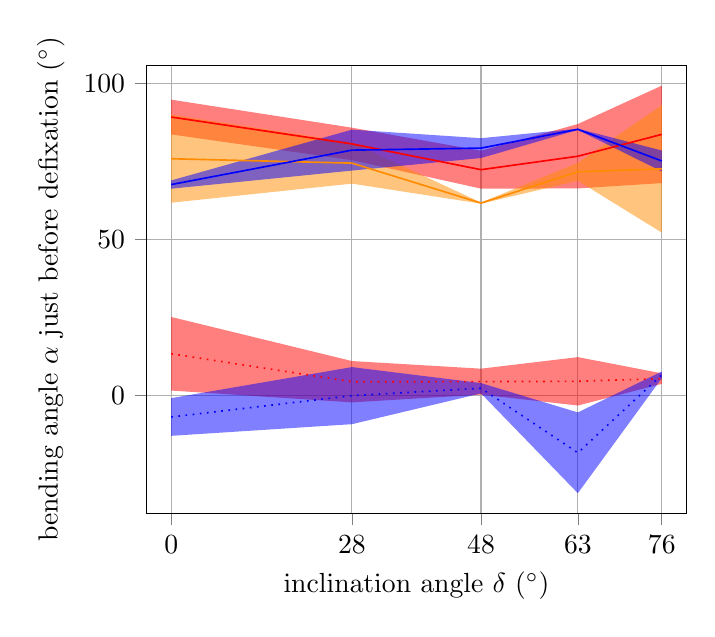
\begin{tikzpicture}

\definecolor{color0}{rgb}{1,0.549019607843137,0}

\begin{axis}[
xlabel={inclination angle $\delta$ ($^\circ$)},
ylabel={bending angle $\alpha$ just before defixation ($^\circ$)},
xmin=-3.8, xmax=79.8,
ymin=-37.8276608877133, ymax=105.921787296751,
tick align=outside,
tick pos=left,
xmajorgrids,
x grid style={lightgray!92.026143790849673!black},
ymajorgrids,
y grid style={lightgray!92.026143790849673!black},
xtick={0, 28, 48, 63, 76}
]
\path [fill=red, fill opacity=0.5] (axis cs:0,83.7458104059282)
--(axis cs:0,94.8938526364343)
--(axis cs:28,85.9085586432681)
--(axis cs:48,78.5121152477769)
--(axis cs:63,87.0780286849384)
--(axis cs:76,99.3877214701844)
--(axis cs:76,68.1321049064672)
--(axis cs:76,68.1321049064672)
--(axis cs:63,66.4312930262516)
--(axis cs:48,66.3710176062507)
--(axis cs:28,75.5023640320752)
--(axis cs:0,83.7458104059282)
--cycle;

\path [fill=color0, fill opacity=0.5] (axis cs:0,61.844168419781)
--(axis cs:0,90.0584251316972)
--(axis cs:28,81.1222272106654)
--(axis cs:48,61.9099956550695)
--(axis cs:63,74.6416351630874)
--(axis cs:76,93.1374896893359)
--(axis cs:76,52.2694051984569)
--(axis cs:76,52.2694051984569)
--(axis cs:63,68.8888216099638)
--(axis cs:48,61.5503370315953)
--(axis cs:28,67.9659749528008)
--(axis cs:0,61.844168419781)
--cycle;

\path [fill=blue, fill opacity=0.5] (axis cs:0,66.3453406465494)
--(axis cs:0,68.9988832410952)
--(axis cs:28,85.268189703038)
--(axis cs:48,82.5373101669754)
--(axis cs:63,85.5769529670002)
--(axis cs:76,78.5972100371633)
--(axis cs:76,71.8898814848968)
--(axis cs:76,71.8898814848968)
--(axis cs:63,85.1965893180437)
--(axis cs:48,76.176324239926)
--(axis cs:28,72.1465382185988)
--(axis cs:0,66.3453406465494)
--cycle;

\path [fill=red, fill opacity=0.5] (axis cs:0,1.62183822961922)
--(axis cs:0,25.2220045725539)
--(axis cs:28,11.0830856557487)
--(axis cs:48,8.63707564638323)
--(axis cs:63,12.3420833333333)
--(axis cs:76,7.14719632389866)
--(axis cs:76,3.76724688326478)
--(axis cs:76,3.76724688326478)
--(axis cs:63,-3.17668875667949)
--(axis cs:48,0.318605422633481)
--(axis cs:28,-2.17132936459835)
--(axis cs:0,1.62183822961922)
--cycle;

\path [fill=blue, fill opacity=0.5] (axis cs:0,-12.895112026036)
--(axis cs:0,-0.81729520851003)
--(axis cs:28,9.14139989115814)
--(axis cs:48,4.00991000781649)
--(axis cs:63,-5.39456141776176)
--(axis cs:76,7.73254665896166)
--(axis cs:76,5.58955211225686)
--(axis cs:76,5.58955211225686)
--(axis cs:63,-31.2935950611467)
--(axis cs:48,0.709411822163024)
--(axis cs:28,-9.16151029709361)
--(axis cs:0,-12.895112026036)
--cycle;

\addplot [semithick, red, forget plot]
table {%
0 89.3198315211813
28 80.7054613376716
48 72.4415664270138
63 76.754660855595
76 83.7599131883258
};
\addplot [semithick, color0, forget plot]
table {%
0 75.9512967757391
28 74.5441010817331
48 61.7301663433324
63 71.7652283865256
76 72.7034474438964
};
\addplot [semithick, blue, forget plot]
table {%
0 67.6721119438223
28 78.7073639608184
48 79.3568172034507
63 85.386771142522
76 75.24354576103
};
\addplot [semithick, red, dotted, forget plot]
table {%
0 13.4219214010866
28 4.45587814557516
48 4.47784053450836
63 4.58269728832692
76 5.45722160358172
};
\addplot [semithick, blue, dotted, forget plot]
table {%
0 -6.85620361727304
28 -0.0100552029677345
48 2.35966091498976
63 -18.3440782394542
76 6.66104938560926
};
\end{axis}

\end{tikzpicture}
%% End matplotlib2tikz content %% 
\end{document}